%generare il pdf con il comando: pdflatex main.tex
\documentclass[a4paper, oneside, openany]{article}
\usepackage{../../template/sos}
\newcommand{\Titolo}{Norme di Progetto}

\newcommand{\Gruppo}{SonsOfSwe}

\newcommand{\Redazione}{Caldart Federico, Cavallin Giovanni, Dalla Riva Giovanni, Favero Andrea, Menegon Lorenzo, Panozzo Stefano, Thiella Eleonora}

\newcommand{\ACapoRedazione}{Caldart Federico \newline Cavallin Giovanni \newline Dalla Riva Giovanni \newline Favero Andrea \newline Menegon Lorenzo \newline Panozzo Stefano \newline Thiella Eleonora}

\newcommand{\Verifica}{Caldart Federico}

\newcommand{\Approvazione}{Cavallin Giovanni}

\newcommand{\Distribuzione}{Vardanega Tullio}

\newcommand{\Uso}{interno}

\newcommand{\Data}{3 Marzo 2018}

\newcommand{\NomeProgetto}{Progetto Speect}

\newcommand{\Mail}{sonsofswe.swe@gmail.com}

\newcommand{\DescrizioneDoc}{Questo documento descrive le regole, gli strumenti e le convenzioni adottate dal gruppo SonsOfSwe durante la realizzazione del progetto Marvin.}



\begin{document}
\copertina{}
%%%%%%%%%%%%%%%%%%%%%%%%%%%%%%%%%%%%%%%%%%%%%%%%%%%%%%%%%%%%%%%%%%%%%%%%%%%%%%%%%%%%%%%%%%%%%%%%%%%%%%%
%SOMMARIO
\tableofcontents
\newpage
%%%%%%%%%%%%%%%%%%%%%%%%%%%%%%%%%%%%%%%%%%%%%%%%%%%%%%%%%%%%%%%%%%%%%%%%%%%%%%%%%%%%%%%%%%%%%%%%%%%%%%%
%PARAGRAFI
\newpage
\section{Introduzione}
\subsection{Scopo del documento}
Questo documento contiene la pianificazione delle attività che saranno svolte dai membri del gruppo \Gruppo{} per realizzare il progetto \NomeProgetto. In particolare, questo documento contiene:

\begin{itemize}
	\item Analisi e trattamento dei rischi;
	\item Il preventivo delle risorse necessarie allo svolgimento del progetto;
	\item Il consuntivo delle attività finora svolte.
\end{itemize}

\subsection{Scopo del prodotto}
Lo scopo del prodotto è quello di realizzare un prototipo di Uniweb come ÐApp che giri su rete Ethereum. I tre attori principali che si rapportano con Marvin sono:
\begin{itemize}
	\item Università;
	\item Professori;
	\item Studenti.
\end{itemize} 
Il portale deve quindi permettere agli studenti di accedere alle informazioni riguardanti le loro carriere universitarie, di iscriversi agli esami, di accettare o rifiutare voti e di poter vedere il loro libretto universitario.
Ai professori deve invece essere permesso registrare i voti degli studenti.
L'università ogni anno crea una serie di corsi di laurea rivolti a studenti, dove ognuno di essi comprende un elenco di esami disponibili per anno accademico. Ogni esame ha un argomento, un numero di crediti e un professore associato. Gli studenti si iscrivono ad un corso di laurea e tramite il libretto elettronico mantengono traccia ufficiale del progresso.

\subsection{Glossario}
Nel documento \textit{Glossario} i termini tecnici, gli acronimi e le abbreviazioni sono definiti in modo chiaro e conciso, in modo tale da evitare ambiguità e massimizzare la comprensione dei documenti.
\newline I vocaboli presenti in esso saranno posti in corsivo e presenteranno una "G" maiuscola a pedice.

\subsection{Riferimenti}
\subsubsection{Normativi}
\begin{itemize}
	\item \textbf{Norme di Progetto: }\textit{Norme di Progetto v1.0.0};
	\item \textbf{Capitolato d'appalto C6: \NomeProgetto}:\\
	\url{http://www.math.unipd.it/~tullio/IS-1/2017/Progetto/C6.pdf};
	\item \textbf{Regolamento del progetto didattico}:\\
	\url{http://www.math.unipd.it/~tullio/IS-1/2017/Dispense/P01.pdf};
	\item \textbf{Vincoli di organigramma e dettagli tecnico-economici}:\\
	\url{http://www.math.unipd.it/~tullio/IS-1/2017/Progetto/RO.html}.
\end{itemize}
\subsubsection{Informativi}
\begin{itemize}
	\item \textbf{Studio di Fattibilità: }\textit{Studio di Fattibilità v1.0.0};
	\item \textbf{Analisi dei Requisiti: }\textit{Analisi dei Requisiti v1.0.0};
	\item \textbf{Software Engineering (10th edition) - Ian Sommerville}:
	\begin{itemize}
		\item Chapter 2: Software processes;
		\item Chapter 22: Project management;
		\item Chapter 23: Project Planning.
	\end{itemize}
	\item \textbf{Slides del corso di Ingegneria del Software}:\\
	\url{http://www.math.unipd.it/~tullio/IS-1/2017/}.
\end{itemize}

\subsection{Modello di sviluppo}
Il modello di sviluppo scelto per il progetto è quello incrementale.\\
Durante i primi periodi, grazie ad un'analisi del capitolato e la comunicazione con il proponente, si fissano i requisiti che il sistema dovrà soddisfare e quali invece sono considerati opzionali, benchè desiderabili. Questo permette di individuare quali dei requisiti hanno una maggior importanza strategica; pertanto questi verranno soddisfatti per primi, mentre gli altri saranno adempiti successivamente.\\
Il modello infatti prevede rilasci multipli successivi, dunque è possibile sottoporre al proponente un prototipo con le funzionalità di primaria importanza nel minor tempo possibile, così da permettere una valutazione in corso d’opera del lavoro svolto. Partendo da questo prototipo sarà poi possibile effettuare un incremento delle funzionalità e un consolidamento di quelle già presenti.\\
Per ottenere ciò nel modo più efficiente ed efficace possibile, si prevede la scomposizione dello sviluppo in attività, al termine delle quali è prevista una milestone (interna o esterna). In questo modo le risorse vengono concentrate in un numero limitato di sottoattività parallele, ottenendo come risultato una loro migliore gestione e verifica.
Questo permette un maggiore controllo sulle tempistiche e sui costi in quanto ogni sottoinsieme deve essere precedentemente pianificato; ciò riduce inoltre il rischio di ritardi.\\
Infine, per ogni attività si prevedono dei giorni di slack prima della consegna dei documenti per accedere alle revisioni di avanzamento, in modo da mitigare eventuali ritardi causati da fattori non prevedibili.

\subsection{Scadenze}\label{Scadenze}
Il gruppo \Gruppo ha deciso di rispettare le seguenti scadenze:
\begin{itemize}
	\item \textbf{Revisione dei Requisiti (RR)}: 23-04-2018;
	\item \textbf{Revisione di Progettazione (RP)}: 14-05-2018;
	\item \textbf{Revisione di Qualifica (RQ)}: 15-06-2018;
	\item \textbf{Revisione di Accettazione (RA)}: 16-07-2018.
\end{itemize}

\section{Obiettivi di qualità}
Questa sezione ha l'obiettivo di definire le caratteristiche riguardanti la qualità di prodotto e di processo che dovranno essere perseguite durante lo sviluppo del progetto.
Ogni caratteristica viene valutata da una metrica, una soglia di accettabilità, ed una possibile soglia di miglioramento che il \emph{team}\ped{G} si prefigge di raggiungere e possibilmente superare.

\subsection{Qualità di processo}
La qualità di processo influenza direttamente il prodotto finale realizzato. É necessario quindi sviluppare un processo in grado di produrre ciclicamente un prodotto di alta qualità. Per questo motivo si è deciso di stabilire le seguenti caratteristiche da rispettare per tutto lo sviluppo del progetto, contemporaneamente a:
\begin{itemize}
\item L'applicazione del \emph{Ciclo di Deming}\ped{G}, o \emph{PDCA}, al fine di perseguire il miglioramento continuo delle attività di processo.
\item L'adesione allo standard ISO/IEC 15504, denominato \emph{SPICE}\ped{G}, al fine di applicare una valutazione oggettiva sulla maturità dei processi.
\end{itemize} 

\subsubsection{Pianificazione}
La pianificazione temporale necessita di uno sguardo a ritroso a partire dagli obiettivi prefissati per completare in tempo adeguato il lavoro previsto. Per un \emph{team}\ped{G} è fondamentale rispettare le scadenze previste, e nel caso in cui si verifichi una situazione di possibile ritardo si rischia di violare l'obiettivo di qualità prefissato, e andranno effettuati quindi dovuti controlli.
\begin{itemize}
	\item \textbf{Metrica}: Si è deciso di utilizzare la \textbf{Schedule Variance}\ped{G}.
	\item \textbf{Soglia di accettabilità}: Si è deciso di ritenere accettabile un ritardo massimo del 10\% rispetto a quanto specificato nel \emph{Piano di Progetto}.
	\item \textbf{Soglia di ottimalità}: Si ritiene un miglioramento rispetto all'obiettivo prefissato il caso in cui un lavoro venga portato a termine in anticipo rispetto a quanto specificato nel \emph{Piano di Progetto}.
\end{itemize}

\subsubsection{Miglioramento}
Al fine di valutare e migliorare la qualità del lavoro svolto è stato assunto il modello di riferimento per la valutazione del livello di maturità definito da SPICE.
\begin{itemize}
	\item \textbf{Metrica}: Verrà utilizzata la struttura a 6 livelli che rappresenta la scala di maturità; la misura di ogni livello sarà effettuata con i 4 livelli N,P,L,F definiti dallo standard.
	\item \textbf{Soglia di accettabilità}: Il livello minimo accettabile di maturità della scala in riferimento ai processi è il 2 (Managed); il processo deve cioè fornire i risultati conformi agli standard ed ai requisiti iniziali in maniera pianificata e tracciabile.
	\item \textbf{Soglia di ottimalità}: La soglia di ottimalità verrà raggiunta con il livello 4 (Predictable); il processo dovrà cioè essere eseguito in conformità ai principi dell'ingegneria del software e attuato all'interno di limiti ben definiti.
\end{itemize}

Per informazioni più approfondite riguardo lo standard ISO/IEC 15504 o SPICE, si rimanda alla sezione~\nameref{AppA:standardProc} dell'appendice A.

\subsubsection{Costo}
Per verificare se i costi sono stati rispettati con quanto concordato nel  \emph{''Piano di Progetto''}, è stato deciso di utilizzare la \emph{\textbf{Cost Variance}}\ped{G} (CV).
Qualora un processo non possieda la qualità minima concordata, necessiterà di lavoro aggiuntivo al fine di soddisfare i requisiti richiesti ma alzando il costo complessivo del progetto, che sarà valutato secondo i seguenti parametri:
\begin{itemize}
	\item \textbf{Metrica}: L'unità di misura scelta per valutare l'aumento dei costi stabiliti è la Cost Variance.
	\item \textbf{Soglia di accettabilità}: Sarà accettabile un aumento dei costi superiore a quelli previsti nel \emph{''Piano di Progetto''} di un massimo del 10\%
	\item \textbf{Soglia di ottimalità}: La soglia di ottimalità verrà raggiunta nel caso in cui i costi non aumenteranno rispetto a quanto concordato nel \emph{''Piano di Progetto''}, 
\end{itemize}

\subsection{Qualità di prodotto}
\subsubsection{Qualità di documento}
Il team si impegna a redigere dei documenti di alta qualità, rispettando le carratestiche di forma e contenuto descritte di seguito.
\paragraph{Ortografia}
Un documento deve essere prima di tutto privo di errori dal punto di vista grammaticale e ortografico. 
Il primo controllo avverà proprio durante la stesura del documento stesso, tramite il sistema di autocontrollo dell'ambiente  \emph{''TexStudio''}, per poi essere controllato una seconda volta dal  \emph{Verificatore}\ped{G}.
\begin{itemize}
	\item \textbf{Metrica}: La quantità di errori riscontrata durante la verifica definitiva del documento sarà l'unità di misura presa in considerazione.
	\item \textbf{Soglia di accettabilità}: Si è accettata come tollerabile la presenza di massimo 3 errori nella seconda e definitiva verifica da parte del \emph{Verificatore}.
	\item \textbf{Sogia di ottimalità}: La soglia di ottimalità verrà raggiunta nel caso in cui dopo la prima revisione del documento non vengano più riscontrati errori dal \emph{Verificatore} e dal \emph{Responsabile}.
\end{itemize}
L'argomento verrà trattato dettagliatamente nella sezione~\nameref{AppB:ErroriOrtografici} in appendice.

\paragraph{Comprensibilità e leggibilità}
Poichè un documento venga considerato leggibile e scorrevole si è deciso di adottare l'\emph{Indice Gulpease}\ped{G}, al fine di avere un parametro oggettivo e facilmente misurabile.
\begin{itemize}
	\item \textbf{Metrica}: L'unità di misura utilizzata è l'\emph{Indice Gulpease}.
	\item \textbf{Soglia di accettabilità}: Verrà considerato come accettabile un valore di 45 sulla scala dell'\emph{Indice Gulpease}.
	\item \textbf{Soglia di ottimalità}: La soglia di ottimalità verrà raggiunta nel caso in cui l'\emph{Indice Gulpease} sia maggiore di 60.
\end{itemize}
L'argomento verrà trattato dettagliatamente nella sezione~\nameref{AppB:IndiceGulpease} in appendice.

\paragraph{Correttezza dei contenuti}
Oltre che ad essere corretto nella forma, un documento necessita di un contenuto adeguato dal punto di vista argomentativo. Gli \emph{Analisti} saranno direttamente responsabili della qualità del contenuto, che poi verrà controllato e corretto dal \emph{Verificatore}.
Per verificare la correttezza concettuale dei documenti prenderemo in esame i seguenti parametri:
\begin{itemize}
	\item \textbf{Metrica}: La quantità di errori di contenuto riscontrata durante la verifica definitiva del documento sarà l'unità di misura presa in considerazione.
	\item \textbf{Soglia di accettabilità}: Si è accettata come tollerabile la presenza di massimo 3 errori nella seconda e definitiva verifica da parte del \emph{Verificatore}.
	\item \textbf{Soglia di ottimalità}: La soglia di ottimalità sarà raggiunta nel caso in cui non si riscontrino errori durante la verifica definitiva del documento.
\end{itemize}

Per maggiori informazioni sulla metrica utilizzata si veda la sezione~\nameref{AppB:ErroriCont} in appendice.

\paragraph{Adesione alle norme interne}
Al fine di ottenere un prodotto coerente ogni documento dovrà essere redatto rispettando strettamente quanto dichiarato nelle \emph{Norme di Progetto}.
Qualunque riferimento non attinente o in contrasto a quanto dichiarato verrà considerato un errore.
\begin{itemize}
	\item \textbf{Metrica}: La quantità di errori di adesione alle norme interne riscontrata durante la verifica definitiva del documento sarà l'unità di misura presa in considerazione. 
	\item \textbf{Soglia di accettabilità}: Si è accettata come tollerabile la presenza di massimo 3 errori nella seconda e definitiva verifica da parte del \emph{Verificatore}.
	\item \textbf{Soglia di ottimalità}: La soglia di ottimalità sarà raggiunta nel caso in cui non si riscontrino errori dopo la prima verifica del documento.
\end{itemize}

Per una precisa definizione degli errori in riferimento alle norme interne si veda la sezione~\nameref{AppB:ErroriForma} in appendice.

\subsubsection{Qualità del software}
Come detto in precedenza, è impossibile distinguere in maniera netta la qualità di processo dalla qualità del software, in quanto la prima influenza direttamente la seconda; è dunque fondamentale avere alla base una qualità di processo sufficientemente buona per garantire la qualità del prodotto. Nonostante ciò, è necessario stabilire degli obiettivi quantitativi di qualità del software oggettivi e misurabili. A tal fine verrà seguito lo standard ISO/IEC 9126, il quale si sostanzia nei sei punti seguenti:

\paragraph{Funzionalità}
È un requisito funzionale che indica la capacità del software di soddisfare le esigenze esposte dal capitolato ed individuate durante l’ \AdR .
Per valutare la funzionalità del software prenderemo in considerazione i seguenti parametri:
\begin{itemize}
	\item \textbf{Metrica}: La valutazione si baserà sul numero di requisiti soddisfatti.
	\item \textbf{Soglia di accettabilità}: Il prodotto verrà valutato come accettabile se tutti i requisiti obbligatori saranno soddisfatti.
	\item \textbf{Soglia di ottimalità}: La soglia di ottimalità sarà raggiunta nel caso in cui siano soddisfatti sia i requisiti obbligatori che tutti i requisiti opzionali.
\end{itemize}

Per maggiori informazioni sulla metrica utilizzata si veda la sezione~\nameref{AppB:Funzionalita} in appendice.


\paragraph{Affidabilità}
È un requisito non funzionale che indica la capacità del software di svolgere correttamente il suo compito, mantenendo delle buone prestazioni anche al variare dell’ambiente nel tempo.
Per valutare l'affidabilità del software prenderemo in considerazione i seguenti parametri:
\begin{itemize}
	\item \textbf{Metrica}: La valutazione si baserà sul numero di fallimenti durante la fase si test.
	\item \textbf{Soglia di accettabilità}: Il prodotto verrà valutato come accettabile se i test falliti saranno inferiori o uguali al 5\%.
	\item \textbf{Soglia di ottimalità}: La soglia di ottimalità sarà raggiunta nel caso in cui il 100\% dei test darà l'esito desiderato.
\end{itemize}

Per maggiori informazioni sulla metrica utilizzata si veda la sezione~\nameref{AppB:Affidabilita} in appendice.

\paragraph{Efficienza}
È un requisito non funzionale che valuta la capacità di un prodotto software di realizzare le funzioni richieste nel minor tempo possibile e con l’uso minimo di risorse necessarie.
\begin{itemize}
	\item \textbf{Metrica}: La valutazione si baserà sui secondi impiegati dal prodotto per eseguire le richieste dell'utente.
	\item \textbf{Soglia di accettabilità}: La soglia di accettabilità è il periodo tra 0 e 10 secondi.
	\item \textbf{Soglia di ottimalità}: La soglia di ottimalità è 1 secondo.
\end{itemize}

Per maggiori informazioni sulla metrica utilizzata si veda la sezione~\nameref{AppB:Efficienza} in appendice.

\paragraph{Usabilità}
L'usabilità è un requisito non funzionale che indica la capacità del software di essere capito e usato correttamente da parte dell'utente finale. Dato che il prodotto finale sarà per l'utente un portale web, è impossibile trovare una metrica quantificabile per valutarne l'usabilità: essa dipende da molteplici fattori che coinvolgono anche le capacità dell'utente stesso e gli strumenti a sua disposizione. Verrà dunque valutata in modo oggettivo basandosi sugli standard del web dichiarati dal \emph{W3C}\ped{G} e sugli strumenti che tale organizzazione mette a disposizione, al fine di creare un'interfaccia web il più accessibile possibile.
Prenderemo in considerazione i seguenti parametri:
\begin{itemize}
	\item \textbf{Metrica}: La valutazione si baserà sul numero di errori trovati dagli strumenti del W3C.
	\item \textbf{Soglia di accettabilità}: La soglia di accettabilità è di 2 errori rilevati.
	\item \textbf{Soglia di ottimalità}: Il prodotto sarà dichiarato ottimo se saranno rilevati 0 errori.
\end{itemize}

Per maggiori informazioni sulla metrica utilizzata si veda la sezione~\nameref{AppB:Usabilita} in appendice.

Quanto detto non assicura però una valutazione completa dell'usabilità, la quale è soggettiva; sarà necessario dunque predisporre test specifici per la misurazione, coinvolgendo ad esempio persone esterne al gruppo al fine di stabilire quanto mediamente il software sia capibile. Al momento il team non è tuttavia in grado di stabilire con precisione una metrica adatta a misurare questo risultato.

\paragraph{Manutenibilità}
La manutenibilità è un requisito non funzionale che indica la capacità di un prodotto di essere evolvibile nel tempo attraverso correzioni, miglioramenti e aggiunte.

\begin{itemize}
\item \textbf{Metrica}: Saranno usate le metriche riguardanti il codice, dato che esso influenza direttamente la manutenibilità del software.
\item \textbf{Soglia di accettabilità}: La soglia di accettabilità sarà raggiunta se il prodotto raggiungerà tale soglia in tutte le metriche utilizzate per il codice.
\item \textbf{Soglia di ottimalità}: La soglia di ottimalità sarà raggiunta se il prodotto raggiungerà tale soglia in tutte le metriche utilizzate per il codice.
\end{itemize}

Per maggiori informazioni sulle metrica per il codice utilizzate si veda la sezione~\nameref{AppB:metricheCod} in appendice.

\paragraph{Portabilità}
La portabilità è un requisito non funzionale che indica la capacità del prodotto di operare in \textit{ambienti}\ped{G} diversi, limitando le necessità di apportare cambiamenti.
\begin{itemize}
	\item Metrica: La valutazione si baserà sul numero di versioni di \emph{browser}\ped{G} e numero di browser stessi su cui il prodotto riesce a venire utilizzato e visualizzato correttamente.
	\item Soglia di accettabilità: La soglia di accettabilità sarà raggiunta se il prodotto sarà supportato correttamente, offrendo la totalità delle sue funzionalità, dalla versione aggiornata dei browser \emph{Google Chrome}\ped{G}, \emph{Microsoft Edge}\ped{G}, \emph{Mozilla Firefox}\ped{G}, \emph{Safari}\ped{G} e \emph{Opera}\ped{G} su \emph{dekstop}\ped{G}.
	\item Soglia di ottimalità: La soglia di ottimalità sarà raggiunta se il prodotto sarà supportato correttamente, offrendo la totalità delle sue funzionalità, in aggiunta ai sopra citati, da \emph{Internet Explorer 11}\ped{G} su desktop e da Google Chrome e Safari nelle versioni \emph{mobile}\ped{G} aggiornate.
\end{itemize}

~\\
Per informazioni più approfondite riguardo lo standard ISO/IEC 9126, si rimanda alla sezione~\nameref{AppA:standardProd} dell'appendice A.




%%%%%%%%%%%%%%%%%%%%%%%%%%%%%%%%%%%%%%%%%%%%%%%%%%%%%%%%%%%%%%%%%%%%%%%%%%%%%%%%%%%%%%%%%%%%%%%%%%%%%%%
\appendix
\pagebreak
\section{Qualità secondo gli standard}
Al fine di perseguire la qualità secondo quanto descritto in questo documento, si è deciso di basarsi su degli standard (descritti qui di seguito) per poter bilanciare la poca esperienza del team con la conoscenza ricavata da anni di pratica nell'ambito dell'ingegneria del software trascritta in tali documenti.
\subsection{Standard di processo: ISO/IEC 15504 - Software Process Improvement and Capability Determination}
\label{AppA:standardProc}
%FONTI:
%http://www.plays-in-business.com/isoiec-15504-spice/
La qualità di un prodotto software dipende dalla qualità dei suoi processi.
L'\emph{ISO/IEC 15504 - Software Process Improvement and Capability Determination} o \emph{SPICE} è uno standard che permette di valutare i processi software di un prodotto con lo scopo di migliorarli  (in modo continuativo). La valutazione dei processi permette di identificare in modo indipendente la \emph{capacità}\ped{G} (capability) di ciascuno di essi attraverso i loro attributi (ovvero gli esiti della valutazione). Basandoci su tali risultati di valutazione (che devono essere comparabili, ripetibili ed oggettivi) ci si può aspettare un miglioramento \emph{continuativo} dei processi e si possono identificare i loro punti di forza, di debolezza ed anche i rischi ed i modi per prevenire questi ultimi.

Ad ogni processo viene assegnato un livello di capacità a seconda della classificazione dei suoi attributi
\begin{labeling}{alligator}
	\item \textbf{0 - Incomplete}: il processo presenta una incapacità generale nel raggiungere il proprio obbiettivo. A questo livello di capacità non viene associato alcun attributo.
	\item \textbf{1 - performed}: il processo è riuscito a raggiungere il proprio obbiettivo. Il raggiungimento di tale obbiettivo potrebbe non essere stato pianificato e tracciato in modo rigoroso. A questo livello è associto l'attributo \textbf{process performance}.
	\item \textbf{2 - managed}: il processo (che appartiene anche al livello 1) rilascia i propri prodotti secondo procedure specifiche ed è pianificato e tracciato. I prodotti sono conformi agli standard specificati ed ai requisiti. A questo livello sono associati due attributi: \textbf{performance management} e \textbf{work product management}.
	\item \textbf{3 - established}: il processo (che appartiene anche al livello 2) viene implementato utilizzando dei buoni principi di ingegneria del software ed è in grado di raggiungere ogni volta che viene eseguito i medesimi risultati. A questo livello sono associati due attributi: \textbf{process definition} e \textbf{process deployment}.
	\item \textbf{4 - predictable}: il processo (che appartiene anche al livello 3) viene eseguito nella pratica in modo coerente rimanendo dentro ai limiti di controllo che, sono stati definiti per raggiungere il suo obbiettivo. Il livello ha associati gli attributi \textbf{process controll} e \textbf{process measurement}
	\item \textbf{5 - optimizing}: le performance del processo (che appartiene anche al livello 4) sono ottimizzate in modo continuo per andare incontro agli obbiettivi ed alle necessità (bisogni) di progetto o di business aziendali presenti e futuri. % I processi raggiungono ''ripetiilità'' nel raggiungere gli obbiettivi di business definiti.
	Anche a questo livello sono associati due attributi: \textbf{process innovation} e \textbf{process optimization}.
\end{labeling}

I 9 attributi che servono per misurare la capacità di un processo sono definiti nel seguente modo:
\begin{labeling}{alligator}
	\item \textbf{Process performance}:  è una misura che indica il raggiungimento degli obbiettivi del processo.
	\item \textbf{Performance management}: è una misura che indica come sono gestite le performance del processo.%The performance management attribute is a measure of the extent to which the performance of the process is managed
	\item \textbf{Work product management}: è una misura che indica quanto i prodotti del processo siano gestiti in modo appropriato.
	\item \textbf{Process definition}: è una misura che indica quanto il processo sia effettivamente impegnato a rispettare gli standard quando produce i propri esiti.
	\item \textbf{Process deployment}: è una misura di quanto il processo standard venga diffuso efficacemente per raggiungere i propri risultati.%The process deployment attribute is a measure of the extent to which the standard process is effectively deployed as a defined process to achieve its process outcomes.
	\item \textbf{Process measurement}:  è una misura che indica quanto vengono usate le misurazioni dei risultati  del processo per assicurarsi che le sue  performance supportino il raggiungimento degli obbiettivi aziendali fissati.
	\item \textbf{Process control}:  è una misura che dà una indicazione di quanto il processo sia gestito in modo quantitativo, questo per produrre un processo che sia stabile, capace\footnote{vedere definizione di \emph{capacità}\ped{G}} e prevedibile entro i limiti definiti.%The process control attribute is a measure of the extent to which the process is quantitatively managed to produce a process that is stable, capable, and predictable within defined limits.
	\item \textbf{Process innovation}: è una misura di quanto i cambiamenti al processo sono identificati grazie ad analisi di cause comuni delle variazioni delle performance e da indagini di approcci innovativi per le definizioni e lo sviluppo dei processi.%The process innovation attribute is a measure of the extent to which changes to the process are identified from analysis of common causes of variation in performance, and from investigations of innovative approaches to the definition and deployment of the process 
	\item \textbf{Process optimization}: è una misura che indica quanto i cambiamenti alla definizione, gestione e performance del processo abbiano un impatto effettivo che permetta di raggiungere gli obiettivi rilevanti di miglioramento del processo.%The process optimization attribute is a measure of the extent to which changes to the definition, management and performance of the process result in effective impact that achieves the relevant process improvement objectives
\end{labeling}

Ogni attributo di processo viene valutato attraverso una scala di valutazione di quattro livelli\footnote{Descritti nella parte 3 dello standard}. Il punteggio è basato sulle prove raccolte tramite degli indicatori che, permettono di sapere in quale livello della classifica si posiziona l'attributo. 
\begin{labeling}{alligator}
	\item \textbf{N - Not achieved}: (0\% - 15\%)
	\item \textbf{P - Partially achieved}: (>15\% - 50\%)
	\item \textbf{L - Largely achieved}: (>50\% - 85\%)
	\item \textbf{F - Fully achieved}: (>85\% - 100\%).
\end{labeling}

Per raggiungere un certo livello di capacità, tutti gli attributi di processo del livello in questione devono essere realizzati almeno come "L" e tutti gli attributi di tutti i livelli di capacità sottostanti devono essere "F".

In Figura~\ref{fig:liv_cap_spice} sono rappresentati gli ultimi cinque livelli di capacità dei processi di SPICE ed i relativi attributi ad essi associati.

\begin{figure}[h!]
	\centering
	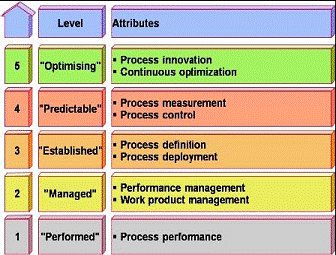
\includegraphics[width=0.50\textwidth]{img/liv_cap_spice.jpg}
	\caption{Ultimi 5 livelli di capacità di SPICE}
	\label{fig:liv_cap_spice}
\end{figure}


\subsection{Standard di prodotto: ISO/IEC 9126}
\label{AppA:standardProd}
Per valutare la qualità del prodotto software si è deciso di utilizzare lo standard ISO/IEC 9126.


É suddiviso in 4 parti:
\begin{labeling}{alligator}
	\item \textbf{Quality Model}: caratteristiche di qualità che possono essere usate per descrivere i fattori di qualità di un prodotto software.
	\item \textbf{External Metrics}: metriche non misurabili direttamente che possono essere usate per valutare se il prodotto software è conforme al modello di qualità.
	\item \textbf{Internal Metrics}: metriche direttamente misurabili utilizzabili per valutare le external metrics.
	\item \textbf{Quality in Use Metrics}: metriche rivolte alla valutazione del sottoinsieme di caratteristiche di qualità legate all’utente.
\end{labeling}

Secondo lo standard sono necessari tre punti di vista per valutare la qualità del prodotto software:
\begin{itemize}
	\item \textbf{percepita/in uso}: è correlata a ciò che percepisce l'utente e per questo motivo definisce delle metriche che possono essere applicate solamente quando il prodotto è finito. Tali metriche esprimono l'efficacia e l'efficienza con cui il software serve le esigenze del suo utilizzatore. 
	 
	\item \textbf{esterna}: rappresenta le prestazioni del prodotto e le funzionalità che esso offre. Definisce delle metriche che esprimono il comportamento dinamico del software, per questo motivo è rilevata attraverso l'analisi dinamica e determina la qualità in uso. É una misura dell'interazione tra il cliente ed il prodotto in un contesto d'uso specifico, permette di osservare il comportamento del software mentre questo viene utilizzato. 
	
	\item \textbf{interna / intrinseca}: rappresenta le qualità intrinseche del prodotto, ovvero quelle misurabili direttamente dal codice sorgente attravero un'analisi di tipo statico. Si realizza partendo dalle specifiche di qualità fornite dall'utente e le specifiche tecniche tradotte dallo sviluppatore nell'architettura del software.
\end{itemize}

Gli attributi di qualità interni, influenzano alcuni degli attributi di qualità esterni e quest'ultimi influenzano quelli della qualità in uso.

Per descrivere i tre punti di vista di cui sopra, lo standard definisce due modelli, uno che riguarda le qualità interna ed esterna, ed un altro che riguarda la qualità in uso. Tali modelli presentano due livelli (primo e secondo) di caratteristiche che definiscono la qualità. Le caratteristiche del secondo livello sono sottocaratteristiche del primo livello e vengono valutate rispetto a delle metriche interne ed esterne. In Figura~\ref{fig:int_ext} e in Figura~\ref{fig:in_use} si possono vedere le caratteristiche associate ai due modelli.

\begin{figure}[h!]
	\centering
	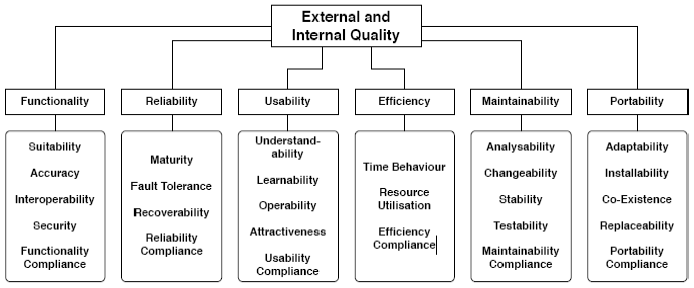
\includegraphics[width=0.50\textwidth]{img/int_ext.png}
	\caption{Caratteristiche associate al modello di qualità interna ed esterna}
	\label{fig:int_ext}
\end{figure}

\begin{figure}[h!]
	\centering
	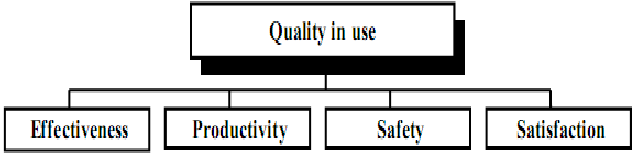
\includegraphics[width=0.50\textwidth]{img/in_use.png}
	\caption{Caratteristiche associate al modello di qualità in uso}
	\label{fig:in_use}
\end{figure}

Di seguito sono elencate le caratteristiche di primo e secondo livello del modello per la qualità interna ed esterna.
\begin{labeling}{alligator}
	\item \textbf{Functionality (funzionalità)}: Il prodotto deve essere in grado di fornire delle funzioni che soddisfino esigenze stabilite (ovvero emerse dall'Analisi dei requisiti).
	\begin{itemize}
		\item \textbf{Suitability (appropriatezza)}: capacità del prodotto di fornire all'utente delle funzioni in grado di soddisfare le esigenze stabilite ed implicite. 
		
		\item \textbf{Accuracy (accuratezza)}: capacità del prodotto di fornire risultati corretti con la precisone richiesta. 
		
		\item \textbf{Interoperability (interoperabilità)}: capacità del prodotto di interagire con uno o più sistemi specificati. 
		
		\item \textbf{Security (sicurezza)}: capacità del prodotto di proteggere i dati e le informazioni in modo che persone/sistemi non autorizzate/i riescano ad accedervi in lettura o scrittura.
		
		\item \textbf{Compliance (conformità)}: capacità del prodotto di aderire agli standard relativi alle funzionalità che offre.
	\end{itemize}
	\item \textbf{Reliability (affidabilità)}: Il prodotto software deve mantenere un livello di prestazioni specificato quando viene eseguito sotto certe condizioni specificate
	\begin{itemize}
		\item \textbf{Maturity (maturità)}: capacità del prodotto di evitare anomalie.
		
		\item \textbf{Fault tolerance (tolleranza all'errore)}: capacità del prodotto di mantenere un livello di prestazioni specificato nel caso occorrano anomalie.
		
		\item \textbf{Recoverability (recuperabilità)}: capacità del prodotto di recuperare un livello di prestazioni specificato ed i dati colpiti da dei malfunzionamenti.
		
		\item \textbf{Compliance (conformità)}: capacità del prodotto di aderire a standard relativi all'affidabilità.
	\end{itemize}
	
	\item \textbf{Usability (usabilità)}: Il prodotto software deve essere compreso ed utilizzato con gradimento dall'utente
	\begin{itemize}
		\item \textbf{Understandability (comprensibilità)}: il prodotto software permette di capire all'utente se può essergli utile per dei compiti particolari.
		
		\item \textbf{Learnability (apprendibilità)}: il prodotto è in grado di far apprendere all'utente come utilizzare le proprie applicazioni.
		
		\item \textbf{Operability (operabilità)}: il prodotto permette all'utente di utilizzarlo e di esercitarne il controllo.
		
		\item \textbf{Attactiveness (attrattività)}: la capacità del prodotto di attrarre l'utente suscitandone un certo livello di gradimento.
		
		\item \textbf{Compliance (conformità)}: la capacità del prodotto di aderire agli standard di usabilità.
	\end{itemize}
	
	\item \textbf{Efficency (efficienza)}: Il prodotto sfrutta al massimo ed al meglio le risorse di cui necessita per espletare le proprie funzioni.
	\begin{itemize}
		\item \textbf{Time behaviour (comportamento nel corso del tempo)}: capacità del prodotto di fornire un tempo di risposta appropriato quando esegue le proprie funzioni.
		
		\item \textbf{Resource utilisation (utilizzo delle risorse)}: la capacità del prodotto di usare la giusta quantità ed il giusto tipo di risorse quando esegue le proprie funzioni.
		
		\item \textbf{Compliance (conformità)}: capacità del prodotto di soddisfare gli standard relativi all'effecienza.
		
	\end{itemize}
	
	\item \textbf{Maintainability (manutenibilità)}: capacità del prodotto di evolversi nel tempo grazie a delle modifiche o correzioni.
	\begin{itemize}
		\item \textbf{Analysability (analizzabilità)}: la capacità del prodotto di essere analizzato per scovare le cause dei malfunzionamenti.
		
		\item \textbf{Changeability (modificabilità)}: la capacità del prodotto di essere modificato.
		
		\item \textbf{Stability (stabilità)}: capacità del software di evitare malfunzionamenti dopo essere stato modificato.
		
		\item \textbf{Testability (testabilità)}: capacità del software modificato di essere verificato e validato.
		
		\item \textbf{Compliance (conformità)}: capacità del prodotto di soddisfare gli standard relativi alla manutenibilità.
	\end{itemize}
	
	\item \textbf{Portability (portabilità)}: Il software deve poter essere trasferito da un ambiente ad un altro con l'avanzare delle nuove tecnologie.
	\begin{itemize}
		\item \textbf{Adaptability (adattabilità)}: la capacità del prodotto di adattarsi ad ambienti diversi senza che ci sia il bisogno di applicare azione alcuna o di utilizzare mezzi diversi da quelli che sono stati già forniti. 
		
		\item \textbf{Installability (instabilità)}: la capacità del prodotto di essere installato in un ambiente specifico.
		
		\item \textbf{Co-existence (coesistenza)}: la capacità del prodotto di coesistere con altri prodotti software indipendenti in uno stesso ambiente condividendone le risorse.
		
		\item \textbf{Replaceability (sostituibilità)}: la capacità del prodotto di sostituire un altro prodotto software con gli stessi scopi nello stesso ambiente. 
		
		\item \textbf{Compliance (conformità)}: capacità del prodotto di soddisfare gli standard relativi alla portabilità.
	\end{itemize}
\end{labeling}

Di seguito sono elencate le caratteristiche del modello per la qualità in uso che, rappresentano il punto di vista dell'utente sulla qualità del prodotto software:

\begin{itemize}
	\item \textbf{Effectiveness (efficacia)}:  permette agli utenti di raggiungere il proprio obbiettivo portandolo a termine con accuratezza e completezza.

	\item \textbf{Productivity (produttività)}: la capacità del prodotto di utilizzare una adeguata quantità di risorse garantendo efficienza.

	\item \textbf{Satisfaction (soddisfazione)}: la capacità del prodotto software di soddisfare gli utenti.

	\item \textbf{Safety (sicurezza)}: la capacità del prodotto di raggiungere livelli accettabili di rischio di danni a persone, software e ambiente operativo su cui è installato.
\end{itemize}

\subsection{Ciclo di Deming}
Il ciclo di Deming, chiamato anche PDCA (Plan, Do, Check, Action.) è uno strumento che permette di realizzare il miglioramento continuo della qualità dei processi e quindi anche dei loro prodotti.

\begin{figure}[h!]
	\centering
	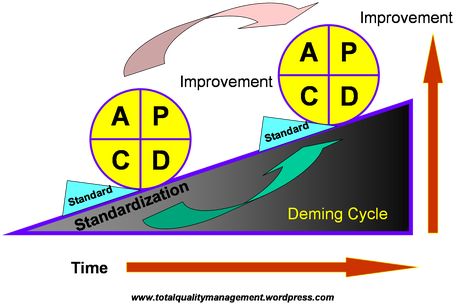
\includegraphics[width=0.50\textwidth]{img/deming.png}
	\caption{Ciclo di Deming}
	\label{fig:PDCA}
\end{figure}

Come si può vedere in Figura~\ref{fig:PDCA} bisogna ripetere in modo iterativo i quattro passi \emph{Plan}, \emph{Do}, \emph{Check} e \emph{Action} per ottenere il miglioramento di un processo.

\begin{itemize}
	\item \textbf{Plan}: vengono pianificati gli obbiettivi per il miglioramento del processo. In questa fase viene analizzata la situazione attuale, vengono raccolti i dati e sviluppate delle metodologie per ottenere dei miglioramenti. Vengono definite le attività che bisogna svolgere, le risorse di cui esse necessitano e si fissano le scadenze.
	
	Per fare ciò è necessario porsi tre domande durante la fase di planning:
	\begin{itemize}
		\item Cosa si sta cercando di realizzare?
		\item Quali cambiamenti si possono fare per ottenere un miglioramento?
		\item Come si è in grado di capire che un dato cambiamento rappresenta un miglioramento?
	\end{itemize}

	\item \textbf{Do}: viene attuato il piano definito nella fase di Plan, in questo modo il processo viene eseguito e così viene creato il prodotto.
	
	\item \textbf{Check}: viene controllato che il processo funzioni come pianificato, in particolare si confrontano i risultati misurati nella fase di Do con gli obbiettivi stabiliti nella fase di Plane (ovvero i risultati attesi).
	
	\item \textbf{Action}: il processo viene migliorato attuando se necessario delle azioni correttive che devono agire sulle differenze riscontrate tra i risultati attesi e quelli misurati.
\end{itemize}

Quando tutte queste quattro fasi vengono portate a termine con il massimo della soddisfazione, il miglioramento viene standardizzato. Il prodotto standardizzato è il risultato dell'iniziativa di miglioramento. É possibile che con il cambiamento di alcune circostanze, il processo sia soggeto ad un nuovo miglioramento, in questo modo il ciclo di deming viene ripetuto di volta in volta.
\pagebreak
\section{Metriche}
\subsection{Metriche per il processo}
\label{AppB:metricheProc}
In questa sezione verranno descritte le metriche che verranno utilizzate per garantire la qualità dei processi.

\paragraph{Schedule Variance - SV}
	~\\La Schedule Variance è un indicatore permette di capire se un processo è il linea con la scheduazione temporale indicata del \emph{Piano di Progetto} o in anticipo o ritardo. Viene calcolata come differenza tra BCWP (Budgeted Cost of Work Performed), cioè il valore, delle attività svolte fino al momento del calcolo e BCWS (Budgeted Cost of Work Scheduled), cioè il valore delle attività che dovrebbe essere state completate secondo la schedulazione preventivata:
	
	\begin{displaymath}
\mbox{SV}= \mbox{BCWP}-\mbox{BCWS}
\end{displaymath}

I risultati possibili sono tre:

\begin{itemize}
\item SV > 0, che indica un anticipo sui tempi pianificati.
\item SV = 0, che indica l'essere in linea con i tempi pianificati.
\item SV < 0, che indica un ritardo sui tempi pianificati.
\end{itemize}

\subparagraph{Soglie}
\begin{itemize}
\item Accettabilità: sarà accettato un valore SV $\ge$ 0.
\item Ottimalità: sarà ottimo un valore SV > 0.
\end{itemize}
	
\paragraph{Cost Variance - CV}
	~\\La Cost Variance è una metrica che permette di capire se i costi effettivi sono in linea o meno con i costi pianificati nel \emph{Piano di Progetto}. Viene calcolata come differanza tra BCWP (Budgeted Cost of Work Performed), cioè il valore delle attività svolte fino al momento del calcolo e ACWP (Actual Cost of Work Performed), cioè il costo effettivamente sostenuto. 
	
	\begin{displaymath}
\mbox{SV}= \mbox{BCWP}-\mbox{ACWP}\end{displaymath}

I risultati possibili sono tre:

\begin{itemize}
\item CV > 0, che indica che il progetto sta producendo con un minor costo rispetto a quanto pianificato.
\item CV = 0, che indica l'essere in linea con i costi preventivati.
\item CV < 0, che indica che il progetto sta producendo con un costo maggiore rispetto a quello pianificato.
\end{itemize}

\subparagraph{Soglie}
\begin{itemize}
\item Accettabilità: sarà accettato un valore CV $\ge$ 0.
\item Ottimalità: sarà ottimo un valore CV > 0.
\end{itemize}

\subsection{Metriche per il prodotto}
\label{AppB:metricheProd}
\subsubsection{Metriche per i documenti}
\label{AppB:metricheDoc}
In questa sezione vengono descritte le metriche che verranno utilizzate nel processo di verifica dei documenti prodotti.
\paragraph{Errori ortografici}
\label{AppB:ErroriOrtografici}
	~\\Questa è la metrica che serve ad esprimere un giudizio di correttezza ortografica riguardo il documento prodotto. Gli errori saranno individuati secondo le seguenti modalità:
il primo controllo avverrà a tempo di stesura del documento tramite lo strumento di autocorrezione dell'ambiente \emph{''TexStudio''}, mentre il secondo controllo avverrà dopo aver terminato la prima redazione del documento stesso, tramite una verifica manuale del \emph{Verificatore}\ped{G}.
Questa metrica misura il numero di errori riscontrati, attraverso le due modalit`a di verifica, ma
non corretti immediatamente.
\newline Formula:
\begin{displaymath}
\mbox{Errori ortografici}= \frac{\mbox{numero errori non corretti}}{\mbox{numero totale errori segnalati}}*100
\end{displaymath}

\subparagraph{Soglie}
\begin{itemize}
\item Accettabilità: valore inferiore o uguale al 5\%.
\item Ottimalità: un valore pari a 0.
\end{itemize}

\paragraph{Indice Gulpease}
\label{AppB:IndiceGulpease}
	~\\L'{Indice Gulpease}\ped{G} è un indice di leggibilità di un testo tarato sulla lingua italiana, con il vantaggio rispetto ad altri indici di utilizzare la lunghezza delle parole in lettere anzichè in sillabe, semplificandone il calcolo automatico. L'indice utilizza due variabili linguistiche: la lunghezza della parola e la lunghezza della frase rispetto al numero delle lettere.
\newline La formula per il suo calcolo è la seguente:
\begin{displaymath}
\mbox{{Indice Gulpease}\ped{G}}= 89+\frac{300*\mbox{(numero delle frasi)}-10*\mbox{(numero delle lettere)}}{\mbox{numero delle parole}}
\end{displaymath}
I risultati sono compresi tra 0 e 100, dove il valore "100" indica la leggibilità più alta e "0" la leggibilità più bassa. In generale risulta che testi con un indice
\begin{itemize}
	\item Inferiori a 80 sono difficili da leggere per chi ha la licenza elementare;
	\item Inferiore a 60 sono difficili da leggere per chi ha la licenza media;
	\item Inferiore a 40 sono difficili da leggere per chi ha un diploma superiore.
\end{itemize}

\subparagraph{Soglie}
\begin{itemize}
\item Accettabilità: un valore superiore o uguale a 45.
\item Ottimalità: un valore compreso tra 75 e 100.
\end{itemize}

\paragraph{Errori contenutistici}
\label{AppB:ErroriCont}
	~\\Questa è la metrica necessaria ad esprimere la correttezza del contenuto di un documento. E' importante verificare che i concetti trattati siano corretti e coerenti con quanto prefissato. Il valore ottenuto da questa metrica rappresenta il numero di errori concettuali che non sono stati corretti dopo esser stati segnalati dal {Verificatore}\ped{G} durante la precedente verifica del documento.
\newline La formula utilizzata per il calcolo degli errori è la seguente:
\begin{displaymath}
\mbox{Errori concettuali}=\frac{\mbox{numero errori non corretti}}{\mbox{numero totale errori segnalati}}*100
\end{displaymath}

\subparagraph{Soglie}
\begin{itemize}
\item Accettabilità:un valore inferiore o uguale al 5\%.
\item Ottimalità: unun valore uguale allo 0\%.
\end{itemize}

\paragraph{Struttura del documento}
\label{AppB:ErroriForma}
	~\\Viene utilizzata questa unità di misura per verificare quanto un documento sia attinente alle regole strutturali descritte nel documento \textit{Norme di Progetto}.
La metrica si basa sul numero di errori segnalati dal \textit{Verificatore} che non sono stati corretti successivamente.
\newline La formula utilizzata per il calcolo degli errori è la seguente:
\begin{displaymath}
\mbox{Errori di forma}=\frac{\mbox{numero errori non corretti}}{\mbox{numero totale errori segnalati}}*100
\end{displaymath}

\subparagraph{Soglie}
\begin{itemize}
\item Accettabilità:un valore inferiore o uguale al 5\%.
\item Ottimalità: unun valore uguale allo 0\%.
\end{itemize}

\subsubsection{Metriche per il prodotto software}
\label{AppB:metricheSoft}
In questa sezione si descrivono le metriche che verranno usate dal gruppo per verificare e garantire la qualità dei prodotti software durante il periodo del progetto. Si sottolinea il fatto che questa sarà solo una prima stesura delle metriche e sarà raffinata nel corso delle varie revisioni, facendo frutto dell'esperienza che verrà acquisita negli intervalli di lavoro tra esse.

\paragraph{Requisiti soddisfatti}
	~\\Tale metrica verrà utilizzata per valutare la funzionalità del software prodotto attraverso una misurazione quantificativa dei requisiti soddisfatti; verranno effettuate due misurazioni differenti, una per i soli requisiti obbligatori e una per tutti.

\begin{description}
\item[Requisiti obbligatori]
	~\\ \begin{displaymath}
		\mbox{ROS}=\frac{\mbox{numero requisiti obbligatori soddisfatti}}{\mbox{numero totale requisiti obbligatori}}
	\end{displaymath}
	
\item[Requisiti obbligatori e facoltativi]
	~\\ \begin{displaymath}
		\mbox{ROFS}=\frac{\mbox{numero requisiti obbligatori soddisfatti} + \mbox{numero requisiti facoltativi soddisfatti}}{\mbox{numero totale requisiti}}
	\end{displaymath}
\end{description}

\subparagraph{Soglie}
\begin{itemize}
\item Accettabilità: il prodotto verrà considerato accettabile quando ROS = 1.
\item Ottimalità: il prodotto verrà considerato ottimale quando ROSF = 1.
\end{itemize}

\paragraph{Successo dei test}
	~\\Tale metrica verrà utilizzata per valutare in parte il livello di affidabilità del prodotto software tramite il calcolo della percentuale di test aventi successo nella fase di verifica.
	\begin{displaymath}
		\mbox{Successo dei test}=\frac{\mbox{numero test aventi successo}}{\mbox{numero totale dei test effettuati}} * 100
	\end{displaymath}
	
	\subparagraph{Soglie}
	\begin{itemize}
	\item Accettabilità: valore maggiore o uguale al 98\%.
	\item Ottimalità: valore uguale a 100\%; tale risultato non sarà comunque indice di affidabilità totale del software: arrivare ad un tale risultato esigerebbe un carico di lavoro troppo elevato.
	\end{itemize}
	
\paragraph{Tempo di risposta}
	~\\Tale metrica verrà utilizzata per valutare l'efficienza del prodotto basandosi sul tempo medio che intercorrà tra la richiesta di una certa funzionalità da parte dell'utente e la risposta del software. Con \textit{tempo medio} si intende la media tra i tempi medi di risposta di tutte le funzionalità: ognuna di esse dovrà essere testata almeno 5 volte ed in condizioni quanto più differenti.
	
	\begin{displaymath}
		\mbox{T\ped{rispostaF}} =\frac{\sum_{k=1}^5 T\ped{test}k}{5}
	\end{displaymath}
	
	\begin{displaymath}
		\mbox{T\ped{rispostaTOT}} =\frac{\sum_{k=1}^n T\ped{rispostaF}k}{n}
	\end{displaymath}
	
	\subparagraph{Soglie}
	\begin{itemize}
	\item Accettabilità: T\ped{rispostaTOT} compreso tra 0 e 10.
	\item Ottimalità: T\ped{rispostaTOT} uguale o minore di 1.
	\end{itemize}
	 
\paragraph{Validazione pagine web}
	~\\Tale metrica verrà usata come tentativo di applicare una metrica oggettiva e misurabile per valutare l'usabilità del prodotto finale; si è usata la parola "tentativo" poichè in effetti l'usabilità e l'accessibilità di un sito web sono due cose distinte, anche se affini: pagine web con contenuto inaccessibile sarnno sicuramente poco usabili. Valutare l'accessibilità attraverso l'analisi del codice prodotto permetterà dunque di fornire una base allo sviluppo di pagine usabili.
W3C offre uno strumento per valutare le pagine \emph{HTML}\ped{G} e uno per i i fogli di stle \emph{CSS}\ped{G}, come dichiarato nelle \emph{Norme di Progetto}: essi riportano il numero e il tipo di errori trovati nei documenti in esame.

\subparagraph{Soglie}
	\begin{itemize}
	\item Accettabilità: Saranno accettati file HTML e CSS con un numero di errori minore o uguale a 5 ognuno. In relazione alla dimensione finale del progetto, si darà anche un limite al numero totale degli errori come somma degli errori di tutti i file; si prevedono inoltre modifiche del limite di 5 errori rilevati (aumento o diminuzione) in corso d'opera.
	\item Ottimalità: Un numero di errori rilevati pari a 0 sarà indice di ottimalità per un file HTML o CSS.
	\end{itemize}
	
\pagebreak
\subsubsection{Metriche per il codice}
\label{AppB:metricheCod}
In questa sezione si elencheranno e descriveranno le metriche utilizzare per valutare la qualità del codice sorgente prodotto; la loro applicazione sarà utilizzata per valutare il grado di manutenibilità del prodotto software.

\paragraph{Complessità ciclomatica}
	~\\La complessità ciclomatica è una metrica utilizzata per misurare la complessità di un software attraverso la valutazione dei suoi metodi, classi e algoritmi. Essa è calcolata utilizzando il grafo di flusso: in esso i nodi corrispondono a gruppi indivisibili di istruzioni, mentre gli archi connettono due nodi se le istruzioni del secondo possono essere eseguite immediatamente dopo quelle del primo.
Questa misurazione sarà utile nella fase di sviluppo per limitare la complessità delle singole parti del software e nella fase di test per capire quanti test diversi saranno necessari per testare adeguatamente il codice.
La misurazione si baserà su un indice numerico intero: valori troppo alti indicano un'eccessiva complessità del codice con conseguente scarsa manutenibilità, mentre valori troppo bassi potrebbero indicare una scarsa efficienza.

\subparagraph{Soglie}
	\begin{itemize}
	\item Accettabilità: valore di complessità compreso tra 1 e 15, purchè per valori tra 10 e 15 sia specificato il motivo di tale complessità.
 	\item Ottimalità: valore di complessità compreso tra 1 e 10.
	\end{itemize}

\paragraph{Commenti per linee di codice}
	~\\Attraverso tale metrica si valuterà il rapporto commenti/linee di codice: una percentuale abbastanza alta di commenti aiuterà la comprensione del sorgente. Verrà misurata come segue:

	\begin{displaymath}
		\mbox{CxSLOC} =\frac{\mbox{Numero linee di commento}}{\mbox{Numero \emph{SLOC}\ped{G}}} * 100
	\end{displaymath}

\subparagraph{Soglie}
	\begin{itemize}
	\item Accettabilità: sarà accettato un valore CxSLOC compreso tra 20 e 25.
	\item Ottimalità: sarà dichiarato ottimale un valore CxSLOC compreso tra 25 e 35.
	\end{itemize}

\paragraph{Parametri per metodo}
	~\\Tale metrica si basa sul numero di parametri formali dei \emph{metodi}\ped{G} per valutare la complessità del codice: un numero elevato potrebbe infatti indicare un livello di complessità troppo alto per i singoli metodi.

\subparagraph{Soglie}
	\begin{itemize}
	\item Accettabilità: saranno accettati metodi con un numero di parametri minore o uguale a 10.
	\item Ottimalità: saranno considerati ottimi metodi con un numero di parametri minore o uguale a 5.
	\end{itemize}

\paragraph{Linee di codice per metodo}
	~\\Tale metrica verrà utilizzata congiuntamente alla precedente (Parametri per metodo) per valutare il grado di complessità di un metodo: controllando il numero di \emph{statement}\ped{G} per ogni metodo è possibile facilitarne comprensione e verifica, spingendo verso una modularizzazione del codice il più ampia possibile. 
Questa metrica sarà fortemente influenzata dall'esperienza che il team guadagnerà durante lo sviluppo del progetto, motivo per cui i valori che seguono saranno indicativi e molto probabilmente modificati in futuro.

\subparagraph{Soglie}
	\begin{itemize}
	\item Accettabilità: saranno accettati metodi con una lunghezza pari o inferiore alle  50 righe.
	\item Ottimalità: saranno considerati ottimi metodi di lunghezza pari o inferiore alle 30 righe.
	\end{itemize}

\paragraph{Copertura del codice}
	~\\Tale metrica è orientata alla valutazione della qualità dei test; essa misura infatti la capacità di coprire mediante test gli statement del codice, attraverso il loro conteggio in percentuale, al fine di fornire dei test che assicurino uan valutazione del software il più affidabile possibile. Verrà calcolata come segue:

	\begin{displaymath}
		\mbox{Copertura} =\frac{\mbox{Numero di statement testati}}{\mbox{Numero di statement totali}} * 100
	\end{displaymath}	
	
\subparagraph{Soglie}
	\begin{itemize}
	\item Accettabilità: sarà accettata un numero di statement testati pari al 70\%.
	\item Ottimalità: sarà considerata ottima la capacità di testare almeno il 90\% degli statement.
	\end{itemize}
	

\paragraph{Copertura dei branch}
	~\\Tale metrica verrà utilizzata congiuntamente alla precedente (Copertura del codice) per valutare la qualità dei test. Essa indicherà la capacità dei test di valutare il maggior numero possibile di rami decisionali del grafo di flusso del software. Verrà calcolata come segue:

	\begin{displaymath}
		\mbox{Copertura\ped{branch}} =\frac{\mbox{Numero di rami raggiunti}}{\mbox{Numero di rami totali}} * 100
	\end{displaymath}	
	
	\subparagraph{Soglie}
	\begin{itemize}
	\item Accettabilità: sarà accettata un numero di rami testati pari al 75\%.
	\item Ottimalità: sarà considerata ottima la capacità di testare almeno il 95\% dei rami per funzionalità non ancora testate, mentre per codice già testato l'ottimalità sara data dalla capacità di testarne l'80\%.
	\end{itemize}


\end{document}


